The field of astrophysical nucleosynthesis can be regarded as starting with the proposal of \cite{eddington1920} that stars have some sort of internal energy source and that the fusion of hydrogen into helium could be that energy source.  Subsequent developments in quantum mechanics revealed how such fusion is possible via quantum tunneling (e.g., \citealt{gurneycondon1928}; \citealt{atkinson1929}). Later, \cite{hoyle1946} and \cite{hoyle1954} discussed the production of elements heavier than helium through fusion inside stars, with $^{56}$Fe being the heaviest element produced.

Figure~\ref{fig:be} shows the binding energy per nucleon as a function of increasing atomic number $A$.  Binding energy per nucleon is minimized for the atomic species $^{56}$Ni (which decays into $^{56}$Fe).  Because of this the fusion of elements heavier than $^{56}$Fe is endothermic and stars cannot maintain such reactions before collapsing.  The nucleosynthesis mechanisms that produce elements heavier than $^{56}$Fe were first explained and predicted in \cite{burbidge1957}.  Among these mechanisms and the focus of this paper are the slow neutron capture process, or s-process, and the rapid neutron capture process, or r-process.  
Since then there has been some debate about the locations where these processes are operative, which will be investigated in Sections~\ref{sec:s} and~\ref{sec:r}.

\begin{figure}
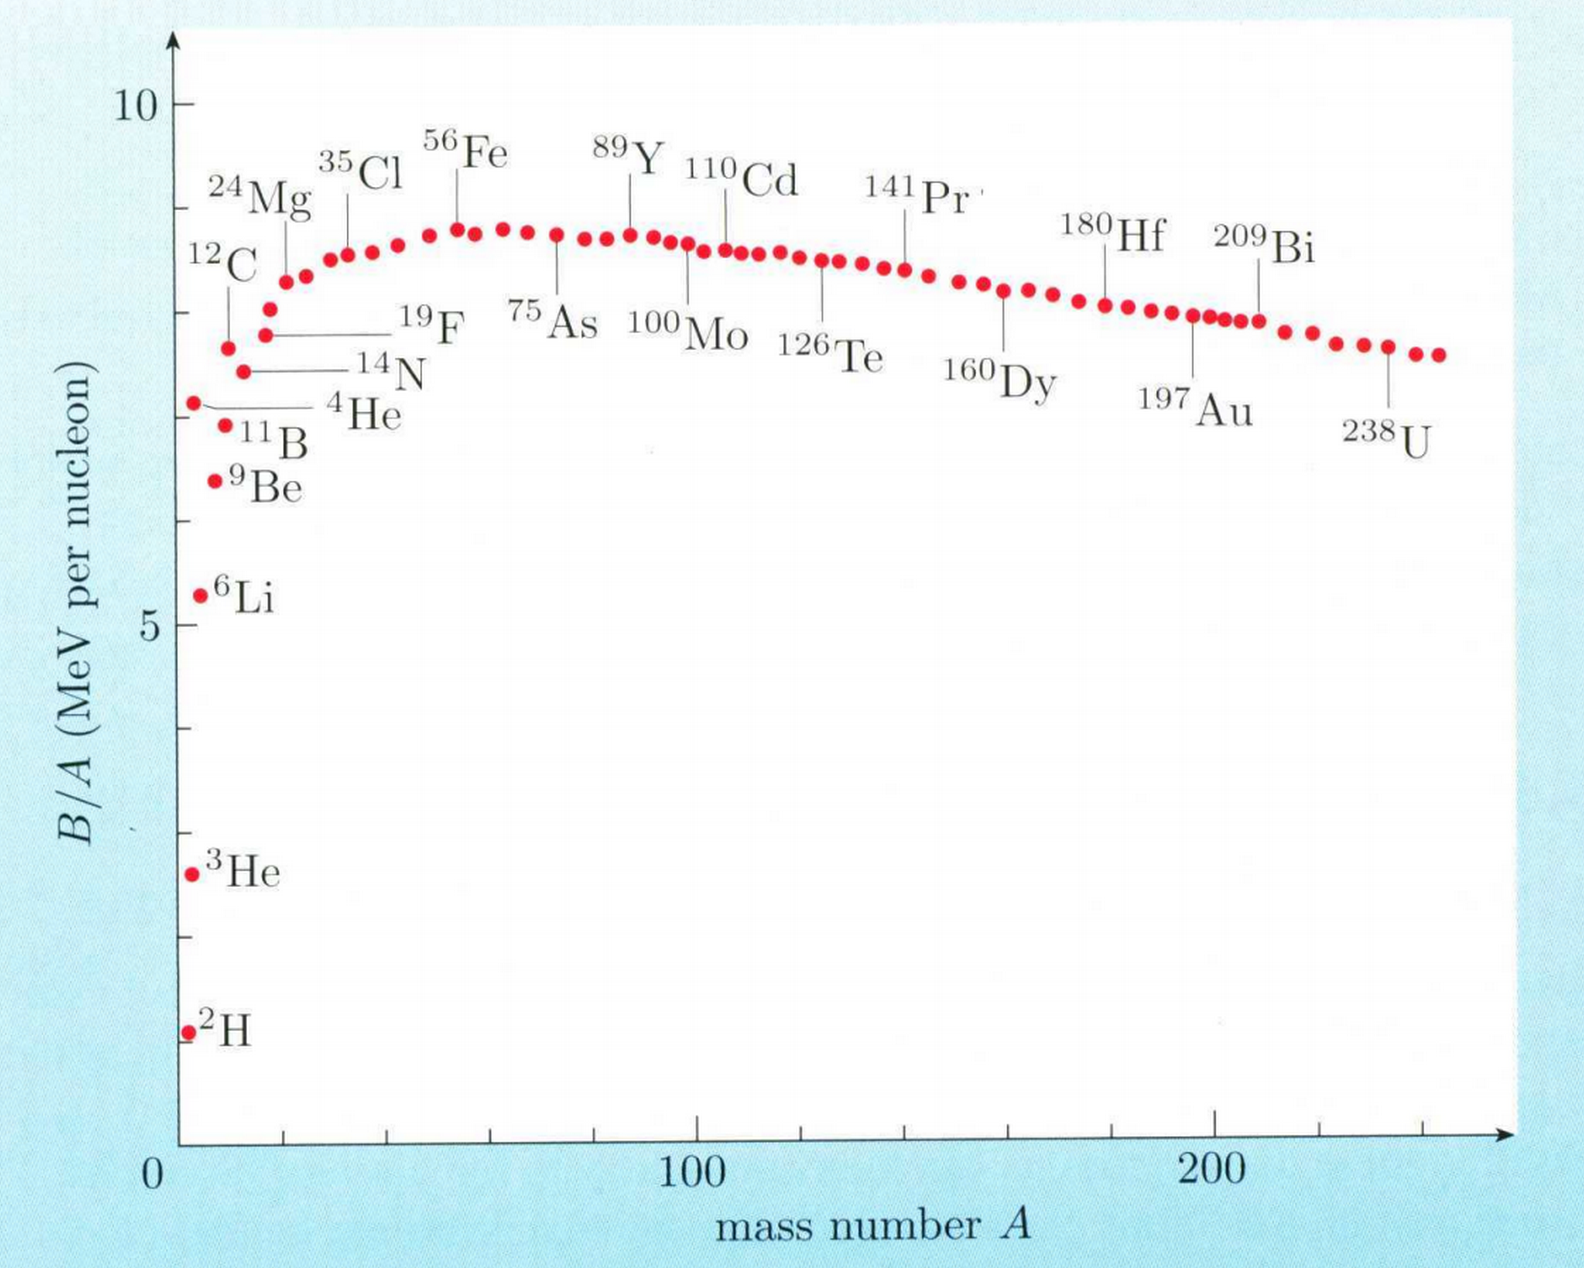
\includegraphics[width=\linewidth]{pdf/bindingenergy.png}
\caption{\label{fig:be}Binding energy per nucleon shown as a function of mass number $A$.  Binding energy per nucleon peaks at $^{56}$Fe.  From~\cite{ryan2010}.}
\end{figure}

%\begin{figure}
%\includegraphics[width=\linewidth]{}
%\caption{\label{} From~\cite{}.}
%\end{figure}

%  LocalWords:  eddington1920 gurneycondon1928 atkinson1929
%  LocalWords:  burbidge1957
